\فصل{راهکار پیشنهادی}

همانطور که در فصل \ref{chapter:c3} مشاهده کردیم، پژوهش‌های زیادی در زمینه حفظ حریم خصوصی در خانه هوشمند انجام شده است اما هر یک نواقصی داشتند. راهکار پیشنهادی این پژوهش، استفاده از تولید رویداد جعلی بر پایه هستی‌شناسی مبتنی بر زمینه به صورت خاص‌دامنه برای خانه‌های هوشمند است تا سکوی نامعتمد، امکان تمایز بین داده‌های حساس کاربر و داده‌های جعلی را نداشته باشد. این رویدادهای جعلی با استفاده از هستی‌شناسی که با استفاده از روش دانش‌محور توسط فرد خبره به برنامه داده شده است، تولید می‌شوند.

\section{توصیف اجمالی}

راهکار ارائه شده با توجه به دسته‌بندی بخش \ref{chapter:c31} یک هستی‌شناسی مبتنی بر زمینه ارائه می‌دهد. هستی‌شناسی در این راهکار شامل نقشه‌ی خانه هوشمند، موقعیت موجودیت‌ها (اشیاء و انسان‌ها) و حالت آن‌ها، فعالیت‌های کاربر و شروط و نتایج هر فعالیت و همچنین فعالیت‌های احتمالی آتی بعد از هر فعالیت می‌باشد. بنابراین، هستی‌شناسی در این راهکار یک هستی‌شناسی مبتنی بر زمینه بوده که به صورت خاص‌دامنه برای خانه‌های هوشمند طراحی شده است.

مدل‌سازی اطلاعات در این راهکار با توجه به دسته‌بندی در بخش \ref{chapter:c32}، با استفاده از روش دانش‌محور می‌باشد زیرا فرد خبره با دانش خود اطلاعات کامل خانه، موجودیت‌ها و فعالیت کاربران را داشته و به برنامه می‌دهد. در این روش شروع سرد نخواهیم داشت و داده‌ها قابلیت استفاده مجدد دارند زیرا در صورت نیاز به استفاده مجدد، تنها بخش کمی از هستی‌شناسی نیاز به تغییر دارد. برای مثال در صورت تغییر منزل توسط کاربران، تنها بخش نقشه خانه و موقعیت موجودیت‌ها در هستی‌شناسی عوض شده و سوابق فعالیت‌های کاربر در هستی‌شناسی ثابت می‌ماند. توجه شود که این راهکار دچار مشکل ناکامل بودن دانش فرد خبره نمی‌شود چرا که برای تولید فعالیت‌های جعلی، نیازی به آگاهی از تمامی فعالیت‌های کاربر نداریم و تنها با داشتن فعالیت‌های روزانه و پرتکرار کاربران، امکان تولید سلسله فعالیت جعلی برای برنامه فراهم است.

در این پژوهش برای حفظ حریم خصوصی در برابر سکوی نامعتمد، با توجه به دسته‌بندی در بخش \ref{chapter:c33}، از راهکار مبتنی بر تولید رویداد جعلی استفاده شده است. با استفاده از هستی‌شناسی مبتنی بر زمینه که شامل سلسله فعالیت‌های کاربران و توالی احتمالی هر دو فعالیت است، برای گمراه کردن سکوی نامعتمد در این پژوهش سلسله فعالیت جعلی مبتنی بر هستی‌شناسی تولید شده که از دید سکو قابل تمایز نباشد. توجه شود که مانند پژوهش ژو و همکاران \cite{x3311}، رویدادهای جعلی با برچسب ارسال می‌شود و کنش‌های مربوط به رویدادهای جعلی کنار گذاشته می‌شوند.

\section{مدل تهدید}\label{chapter:c42}

در این پژوهش، سکوی اینترنت اشیاء صادق ولی کنجکاو فرض شده است و دسترسی به تمامی رویدادهای ارسال شده از حسگرهای خانه هوشمند را داشته و به طور کامل آن‌ها را به همراه زمان دریافت داده از حسگر، ذخیره می‌کند. این ذخیره‌سازی برای آن است که در صورت دریافت سلسله فعالیت جدید کاربران، داده‌های ذخیره شده را با داده‌ی دریافت شده مقایسه کرده و در صورت شباهت بیش از حد، مشکوک به جعلی بودن سلسله فعالیت دریافتی شود.

همچنین سکو به هستی‌شناسی کامل خانه دسترسی داشته و از روابط و همبستگی‌های بین موجودیت‌ها (ناشی از انواع کانال‌های ارتباط دهنده)، متغیرهای محیطی و احتمال سلسله فعالیت‌های مختلف کاربران برای تشخیص واقعی و یا جعلی بودن رویدادها استفاده می‌کند اما با توجه به تغییرات زیاد و پیچیدگی جزئیات خانه هوشمند، از حالت کنونی خانه و موقعیت و حالات موجودیت‌ها اطلاعی ندارد.

برای آن که سکو مشکوک به جعلی بودن یک سلسله فعالیت نشود، نیاز است تا تولید آن سلسله فعالیت با توجه به هستی‌شناسی خانه انجام شده و برای یکسان نبودن هر دو سلسله از فعالیت‌های جعلی، ریز فعالیت‌های انجام شده و همچنین فواصل زمانی بین انجام فعالیت‌ها، به صورت تصادفی انتخاب شده تا سکو با مقایسه‌ی سلسله فعالیت با داده‌های قبلی، متوجه شباهت زیاد بین آن‌ها نشود.

\section{راهکار پیشنهادی}

راهکار ارائه شده در این پژوهش، به حفظ حریم خصوصی کاربران در برابر سکوی نامعتمد بر اساس ترجیحات حریم خصوصی کاربر می‌پردازد. در ادامه به بررسی معماری این راهکار خواهیم پرداخت.

\subsection{معماری کلان}

ابزار مبتنی بر راهکار پیشنهادی این پژوهش مطابق شکل \ref{fig:fxyz}، بین هاب و سکوی اینترنت اشیاء قرار دارد که هر کاربر، فعالیت‌های حساس خود و همچنین فعالیت‌های‌ جعلی جایگزین را اعلام کرده است تا در صورت انجام آن فعالیت‌های حساس، سلسله فعالیت جعلی مبتنی بر نیاز کاربر تولید شود. هر‌ فعالیت موجود در سلسله فعالیت جعلی تولید شده توسط ابزار مبتنی بر راهکار پیشنهادی، در زمان مشخص، رویداد مورد نیاز را از جانب حسگر مربوطه به سکو ارسال می‌کند.

\begin{figure}[htp]
\centerline{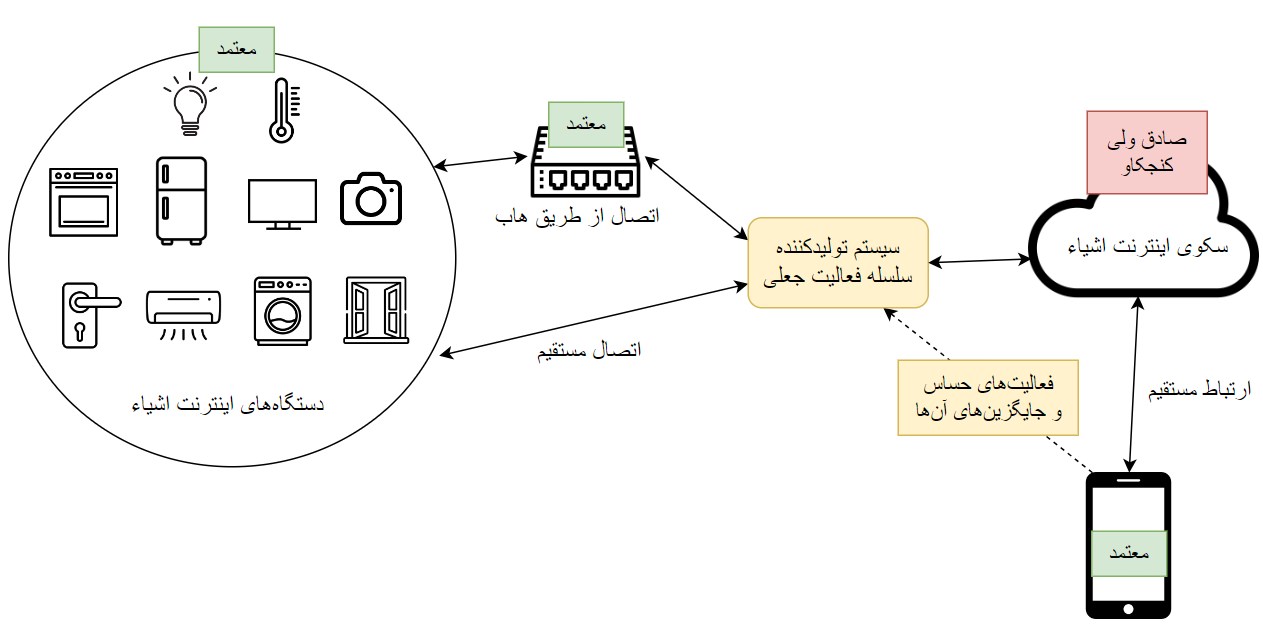
\includegraphics[width=1\textwidth]{figs/fxyz.png}}
\caption{محل استقرار سیستم تولیدکننده سلسله فعالیت جعلی}
\label{fig:fxyz}
\end{figure}

از طرفی، زمانی که سکو دستور کنش‌های مورد نیاز برای رویدادهای دریافتی را ارسال می‌کند؛ ابزار مبتنی بر راهکار پیشنهادی، تمامی کنش‌ها را بررسی کرده و هر کنش که در جواب رویدادی با برچسب جعلی آمده باشد را کنار می‌گذارد تا کارایی خانه هوشمند کاهش پیدا نکند. ابزار مبتنی بر راهکار پیشنهادی، نتایج هر یک از فعالیت‌های کاربر و پاسخ سکو به فعالیت‌ها را به طور کامل می‌داند و هنگام تولید سلسله فعالیت جعلی و ارسال به سکو، آن‌ها را در حافظه موقتی و پرسرعت ذخیره کرده تا در زمان دریافت پاسخ سکو که تقریبا زیر یک ثانیه است، آن پاسخ را در حافظه موقت بررسی کرده و در صورتی که پاسخ یکی از فعالیت‌های جعلی باشد، آن را به خانه‌ هوشمند ارسال نمی‌کند.

کاربر برای تولید سلسله فعالیت جعلی دلخواهش، یکی از دو نوع ورودی \underline{مبتنی بر فعالیت} و \underline{مبتنی بر نتیجه} را به عنوان ورودی به ابزار مبتنی بر راهکار پیشنهادی می‌دهد. حال ابزار مبتنی بر راهکار پیشنهادی، یک سلسله فعالیت جعلی تولید می‌کند که فعالیت جعلی مدنظر کاربر در آن وجود داشته باشد.

از طرفی اگر درخواست کاربر، تولید سلسله فعالیت جعلی بر اساس نتیجه باشد، ابزار مبتنی بر راهکار پیشنهادی در ابتدا تمامی فعالیت‌های منتهی به آن نتیجه را پیدا کرده و سپس بر اساس یکی از آن فعالیت‌ها یک سلسله فعالیت جعلی تولید می‌کند که آن فعالیت را شامل باشد و نتیجه‌ی مدنظر کاربر از فعالیت مذکور گرفته شود. به عنوان مثال زمانی که ترجیح کاربر تولید سلسله فعالیت جعلی مبتنی بر نتیجه‌ی «افزایش نور محیط» است؛ نرم‌افزار ابتدا فعالیت‌های «باز کردن پنجره» (به شرط روز بودن) و «روشن کردن تلویزیون» پیدا کرده، سپس، به صورت تصادفی، یکی از آن‌ها را انتخاب کرده و بر اساس آن فعالیت، یک سلسله فعالیت جعلی شامل فعالیت انتخاب شده تولید می‌کند.

خروجی هر بار اجرای ابزار مبتنی بر راهکار پیشنهادی، یک سلسله فعالیت جعلی بوده که هر یک در زمان خاصی باید از جانب حسگر مربوطه به سکو ارسال شوند. به طور مثال یک سلسله فعالیت جعلی شامل «باز کردن درب پذیرایی در زمان 00:01:40:10» و «روشن کردن کولر در زمان 50:02:40:10» است که بدین معناست که در زمان 00:01:40:10، کاربر درب پذیرایی را باز کرده و در زمان 50:02:40:10، کولر را روشن می‌کند. ابزار مبتنی بر راهکار پیشنهادی برای این سلسله فعالیت جعلی، در زمان 00:01:40:10، رویداد باز شدن درب پذیرایی را از جانب حسگر درب پذیرایی به سکو ارسال می‌کند؛ سپس رویداد روشن شدن کولر را در زمان 50:02:40:10، یعنی یک و نیم ثانیه پس از باز شدن درب پذیرایی، از جانب کولر به سکو ارسال می‌کند.

\section{مدل‌سازی}\label{chapter:c44}

برای مدل‌سازی جامع و کامل در برنامه‌ی این پژوهش، نیاز به هستی‌شناسی مبتنی بر زمینه به صورت خاص‌دامنه برای خانه هوشمند داریم و سپس با استفاده از این هستی‌شناسی اقدام به تولید سلسله فعالیت جعلی می‌نماییم.

\subsection{هستی‌شناسی}

در این پژوهش، هستی‌شناسی که با دانش فرد خبره به صورت دانش‌محور داده شده است؛ در چند بخش مختلف قرار می‌گیرد که در ادامه به توضیحات هر بخش خواهیم پرداخت.

\begin{itemize}
\item \textbf{خانه هوشمند}: همانطور که در شکل \ref{fig:f41} قابل مشاهده است، نقشه‌ی خانه هوشمند توسط فرد خبره تعریف شده است. هر بخش شامل نام و لیست بخش‌هایی از خانه هوشمند است که به طور مستقیم به بخش مورد نظر متصل هستند (به عنوان مثال اتاق خواب، به طور مستقیم به راهرو و بالکن متصل است). استفاده از نقشه‌ی خانه در این پژوهش طوری تعریف شده است که با تغییر نقشه‌ی خانه، نیازی به تغییر دیگری در برنامه نخواهیم داشت و عملکرد برنامه تحت تاثیر قرار نخواهد گرفت.

\begin{figure}[htp]
\centerline{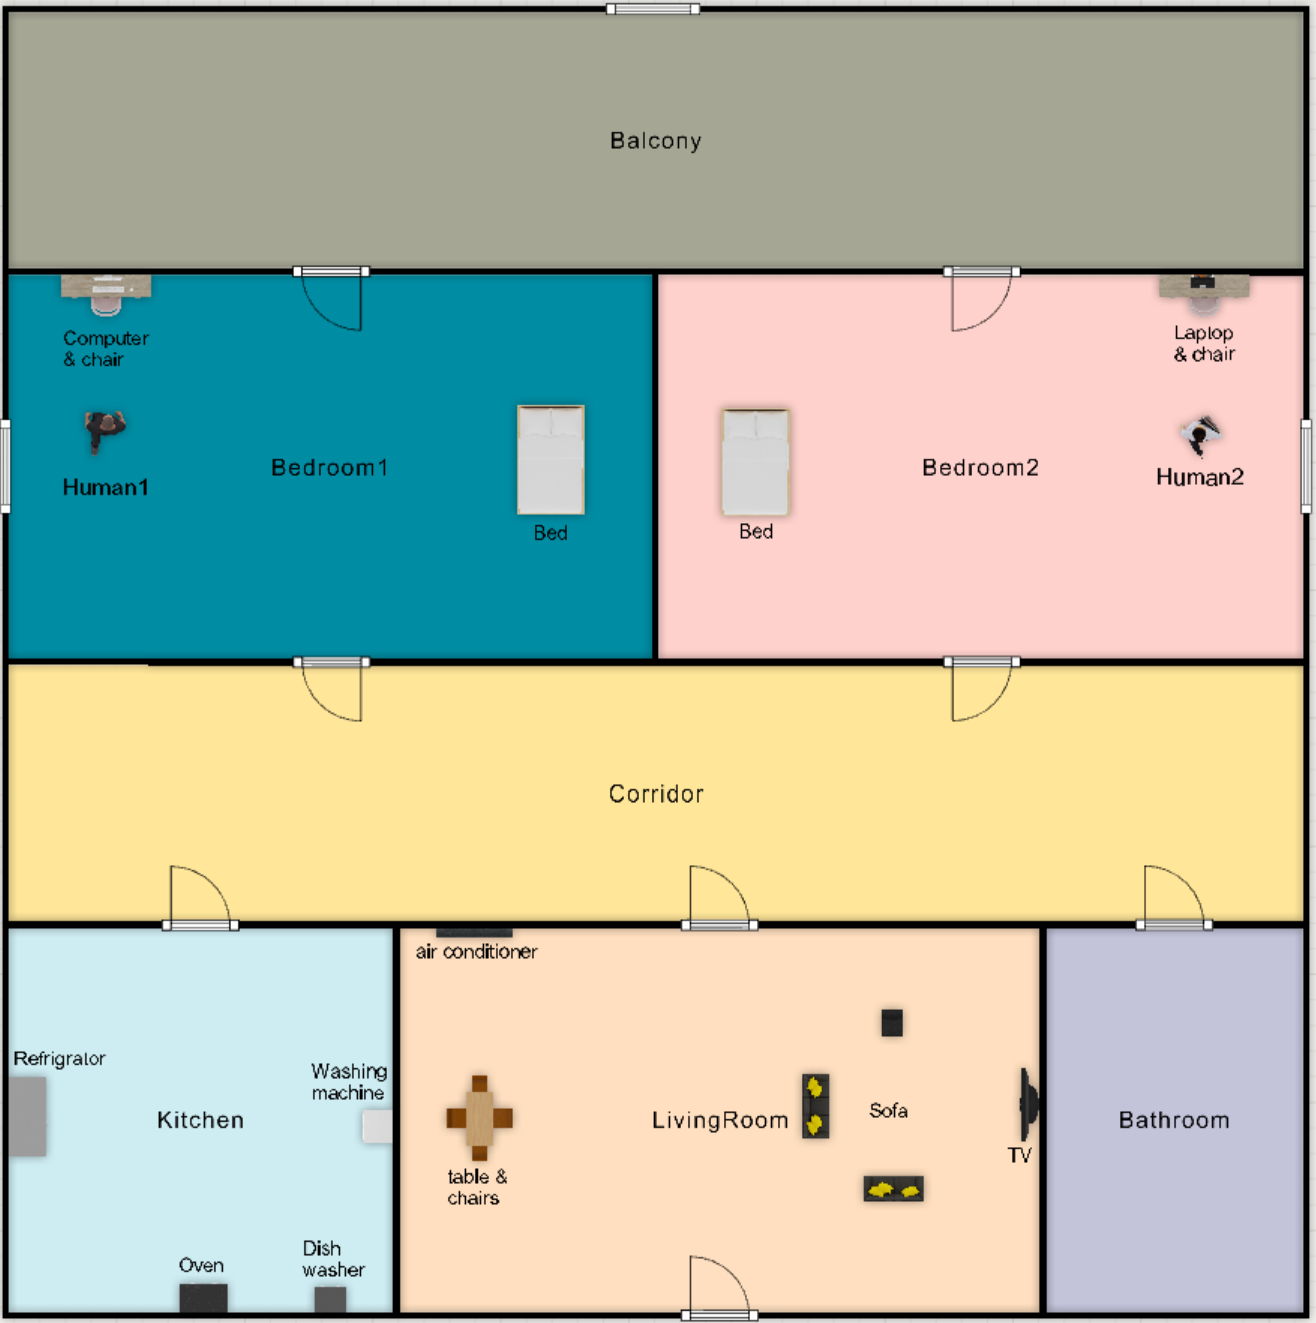
\includegraphics[width=1\textwidth]{figs/f41.png}}
\caption{نمونه نقشه خانه هوشمند}
\label{fig:f41}
\end{figure}

 هستی‌شناسی تعریف شده برای خانه هوشمند، در شکل \ref{fig:f401} قابل مشاهده است. در این هستی‌شناسی هر بخش خانه هوشمند مانند آشپزخانه، راهرو، پذیرایی، بالکن، دستشویی و اتاق‌خواب‌ها و همچنین همسایگان هر کدام، توسط فرد خبره مشخص شده اند.

\begin{figure}[htp]
\centerline{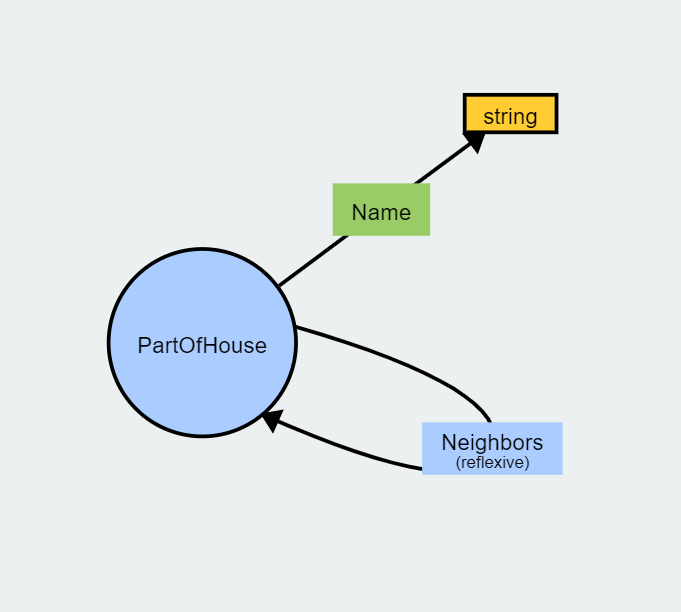
\includegraphics[width=1\textwidth]{figs/f401.png}}
\caption{هستی‌شناسی بخش‌های خانه هوشمند}
\label{fig:f401}
\end{figure}

\item \textbf{موجودیت‌ها}: در هستی‌شناسی که توسط فرد خبره به برنامه داده می‌شود، موقعیت و حالت اولیه برای تمامی موجودیت‌ها (انسان‌ها و اشیاء که حسگر دارند) فراهم می‌شود. در صورتی که در سلسله فعالیت‌های جعلی، موقعیت یا حالت یک موجودیت تغییر کند، این تغییر در پایگاه داده ذخیره می‌شود تا سلسله فعالیت‌های بعدی بر اساس اطلاعات جدید موجودیت‌ها باشد تا از دید سکوی نامعتمد، تناقضی در داده‌ها رخ ندهد اما کنش‌های مربوط به تمامی رویدادهایی که با برچسب جعلی به سکو ارسال شده‌اند، کنار گذاشته می‌شوند تا بهره‌وری خانه هوشمند کاهش پیدا نکند. هستی‌شناسی اشیاء خانه هوشمند در شکل \ref{fig:f402}  و هستی‌شناسی افراد حاضر در خانه در شکل \ref{fig:f403} قابل مشاهده است.

\begin{figure}[htp]
\centerline{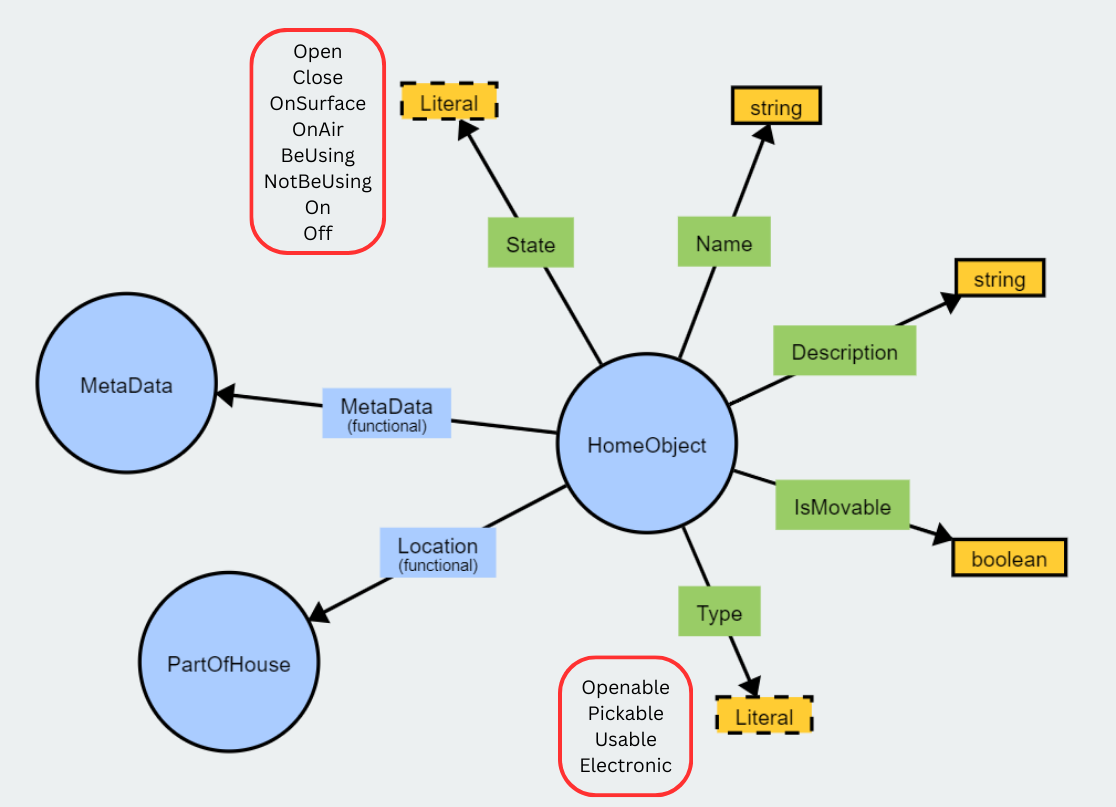
\includegraphics[width=1\textwidth]{figs/f402.png}}
\caption{هستی‌شناسی اشیاء خانه هوشمند} 
\label{fig:f402}
\end{figure}

\begin{figure}[htp]
\centerline{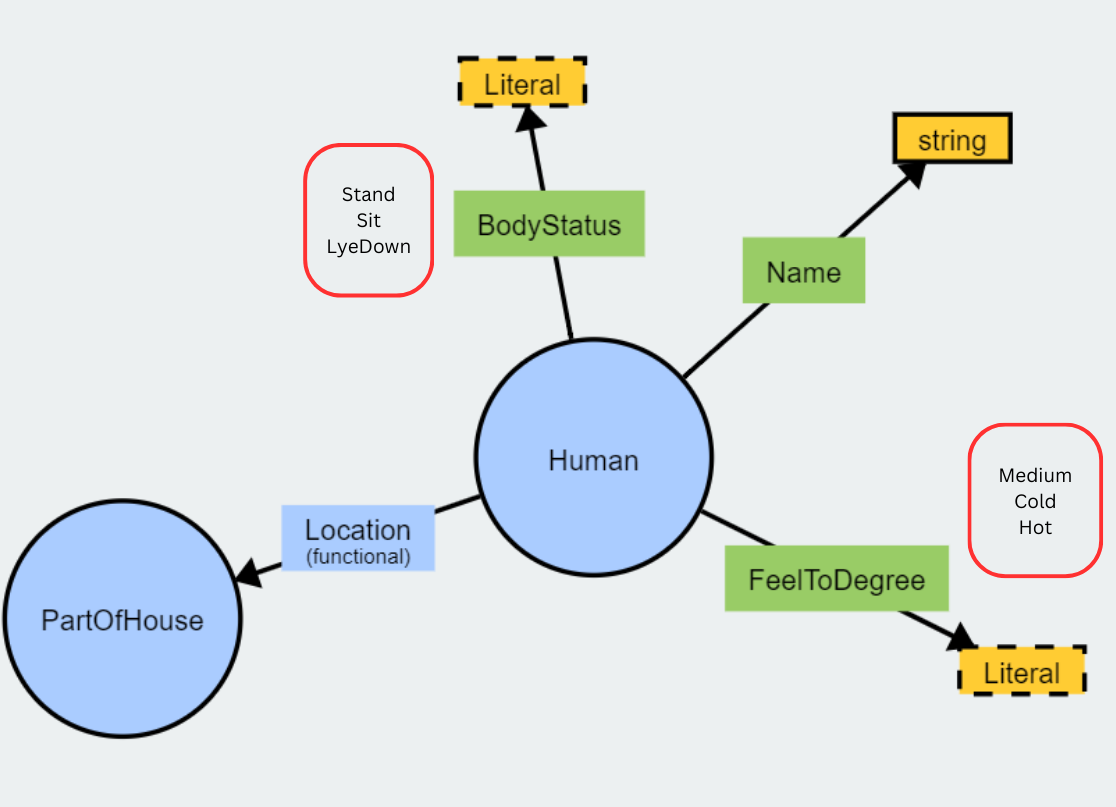
\includegraphics[width=1\textwidth]{figs/f403.png}}
\caption{هستی‌شناسی افراد حاضر در خانه هوشمند}
\label{fig:f403}
\end{figure}

همچنین هستی‌شناسی فراداده‌های اشیاء خانه هوشمند در شکل \ref{fig:f402_metadata} قابل مشاهده است. هر یک از اشیاء خانه هوشمند حداکثر یکی از این فراداده‌ها را در هستی‌شناسی خود دارند تا با استفاده از آن‌ها شروط هر یک از اشیاء به طور دقیق‌تر بررسی شود و تغییر حالت آن به طور دقیق‌تر اعمال شود.

\begin{figure}[htp]
\centerline{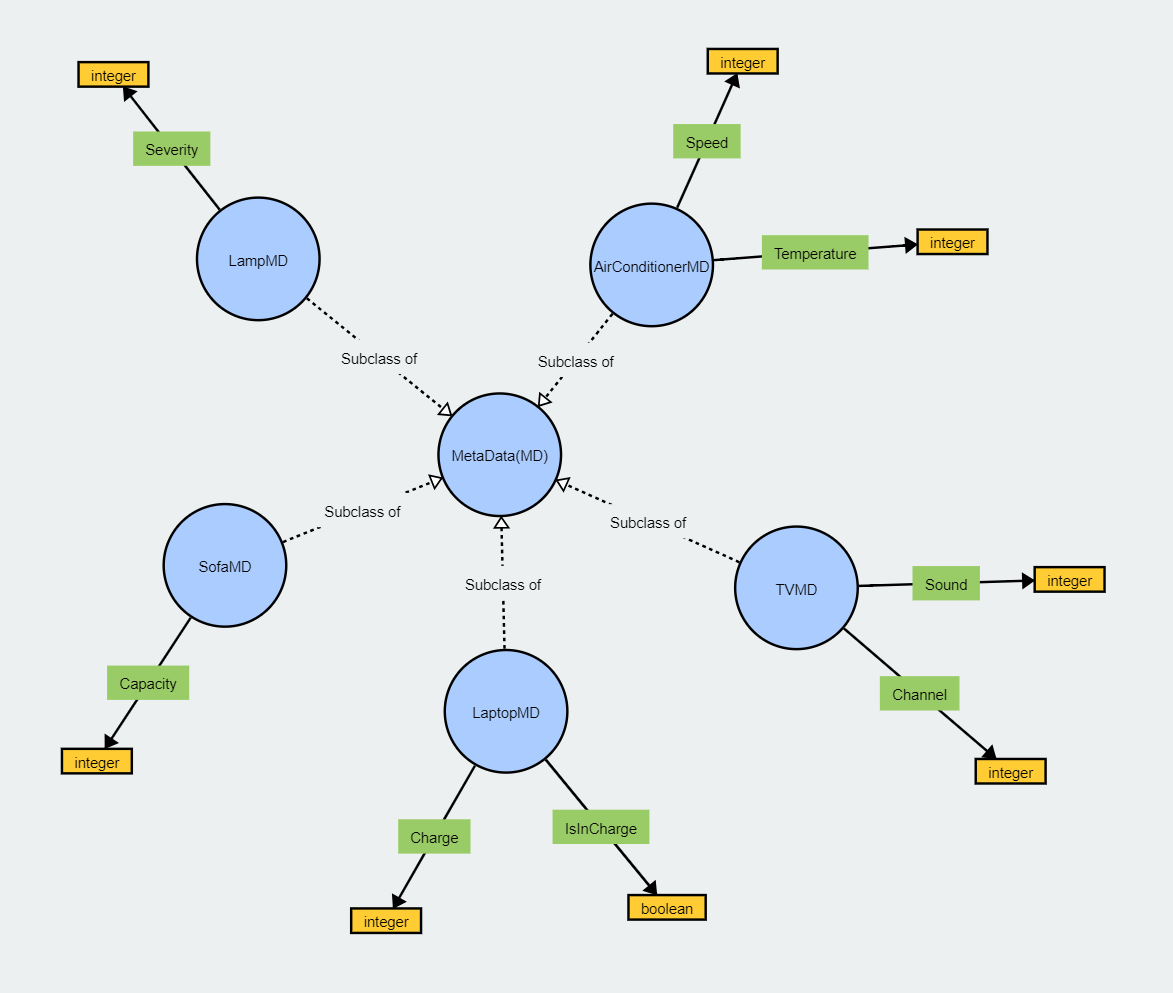
\includegraphics[width=1\textwidth]{figs/f402_metadata.png}}
\caption{هستی‌شناسی فراداده‌های اشیاء خانه هوشمند} 
\label{fig:f402_metadata}
\end{figure}

\item \textbf{شرایط محیطی}: برای دخیل کردن شرایط محیطی مانند میزان نور، دما، صدا و ... در تولید سلسله فعالیت‌های جعلی، مقدار اولیه برای اجزای محیط در دانش اولیه‌ی برنامه قرار دارد. توجه شود که تاریخ و ساعت به عنوان یک متغیر محیطی در تولید سلسله فعالیت جعلی دخیل بوده اما در هستی‌شناسی اولیه قرار ندارد چرا که متغیر زمان به صورت خودکار مقدار می‌گیرد. استفاده از این اجزای محیط کمک به واقعی به نظر رسیدن سلسله فعالیت‌های جعلی خواهد کرد. به عنوان مثال زمانی که پنجره باز می‌شود، حسگر سنجش نور محیط، در ساعاتی که خورشید در آسمان است، رویداد افزایش نور محیط را ارسال می‌کند. پس زمانی که به صورت جعلی ارسال رویداد باز شدن پنجره را به حسگر مربوطه ارسال می‌کنیم، برنامه با توجه به ساعت شبانه روز تصمیم به ارسال یا عدم ارسال رویداد افزایش نور محیط توسط حسگر سنجش نور می‌گیرد. هستی‌شناسی مربوط به اجزای محیط در شکل \ref{fig:f404} قابل مشاهده است.

\begin{figure}[htp]
\centerline{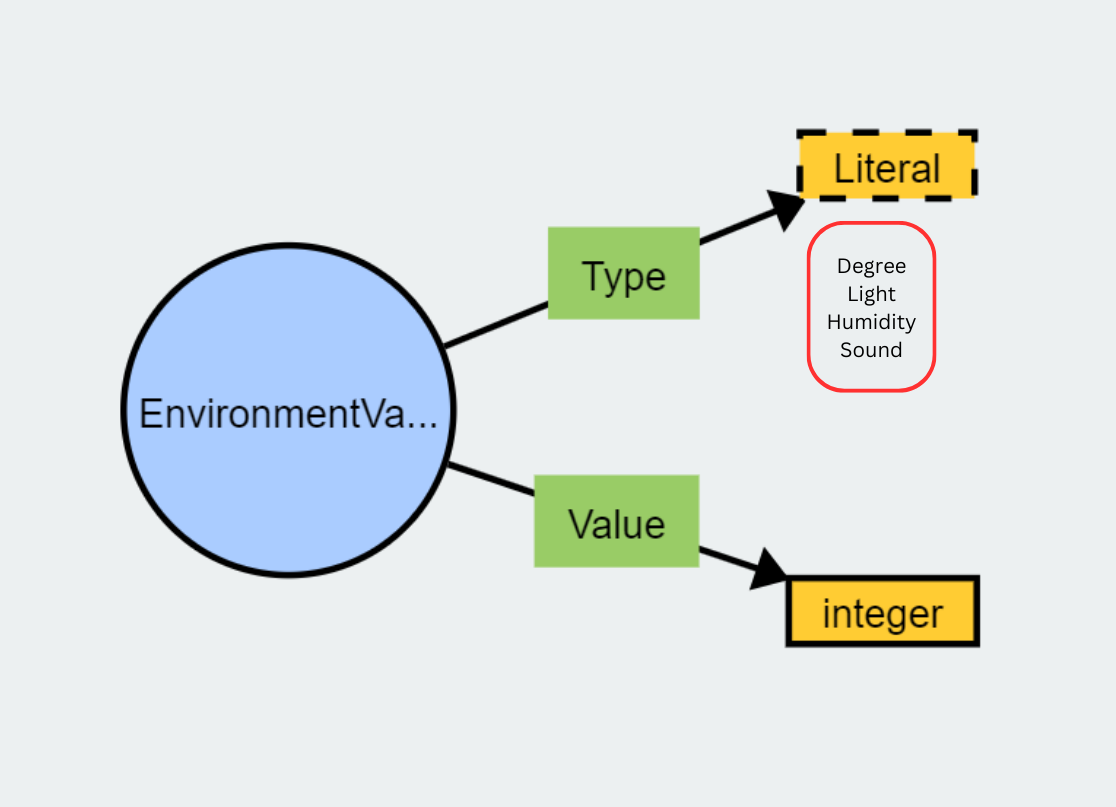
\includegraphics[width=1\textwidth]{figs/f404.png}}
\caption{هستی‌شناسی اجزای محیط خانه هوشمند}
\label{fig:f404}
\end{figure}


\item \textbf{فعالیت}: هر فعالیت کاربر به صورت سابقه‌ی مختص به آن کاربر در هستی‌شناسی اولیه توسط فرد خبره داده می‌شود که فعالیت‌ها شامل شروط مورد نیاز برای انجام به صورت جعلی (به عنوان مثال حضور در پذیرایی برای «روشن کردن تلویزیون»)، نتایج اعمال شده پس از ارسال رویداد جعلی یک فعالیت به سکو (به عنوان مثال کاهش دمای محیط پس از «روشن کردن کولر») و فعالیت‌های احتمالی انجام شده توسط کاربر پس از انجام یک فعالیت مشخص (به عنوان مثال پس از «ورود به پذیرایی»، «روشن کردن کولر» با احتمال 70\% و «نشستن روی مبل» با احتمال 30\% انجام می‌شود) است که نحوه مدل‌سازی احتمال توالی فعالیت‌ها را در بخش \ref{chapter:c442} توضیح خواهیم داد. دانش فرد خبره در این بخش محدود به نوع فعالیت و شروط و نتایج آن‌هاست و احتمال توالی فعالیت‌ها با استفاده از قوانین انجمنی توسط ابزار مبتنی بر راهکار پیشنهادی محاسبه خواهد شد که با استفاده از سوابق موجود از حسگرها به دست می‌آید. توجه شود که هر فعالیت با احتمالی مشخص با توجه به سوابق کاربر، می‌تواند آخرین فعالیت یک سلسله فعالیت جعلی باشد و لزوما نیاز به ادامه در تولید سلسله فعالیت جعلی با توجه به فعالیت احتمالی بعدی نداریم. هستی‌شناسی کلی فعالیت‌ها در شکل \ref{fig:f405} قابل مشاهده است. 

به عنوان مثال در فعالیت «روشن کردن تلویزیون» به عنوان \lr{ActionAggregate}، حضور در پذیرایی یکی از شروط انجام آن (\lr{ActionCondition})، تغییر وضعیت تلویزیون به حالت روشن یکی از نتایج انجام آن (\lr{ActionResult})، افزایش یا کاهش صدای تلویزیون یکی از فعالیت‌های احتمالی بعدی (\lr{NextAction})، "روشن کردن تلیویزیون" نام آن، تاخیر برابر 4 ثانیه، احتمال 50 درصد بودن فعالیت نهایی و "روشن کردن تلویزیون به صورت دستی توسط افراد حاضر در خانه" به عنوان توضیحات بر اساس هستی‌شناسی این فعالیت داده شده است.

\begin{figure}[htp]
\centerline{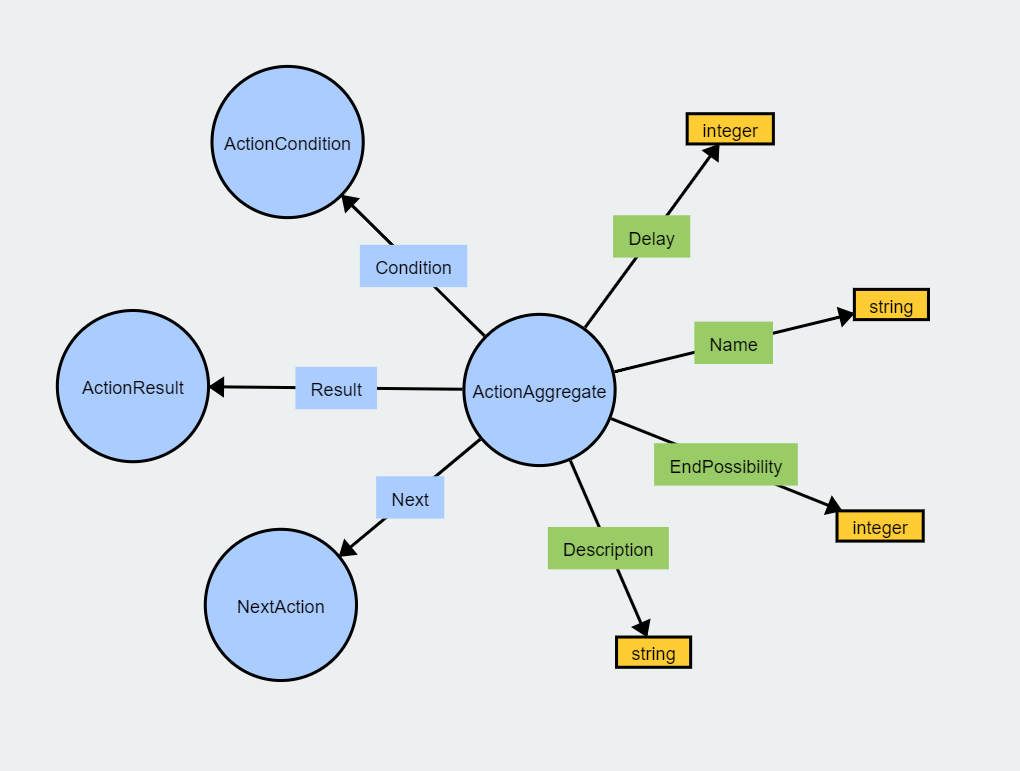
\includegraphics[width=1\textwidth]{figs/f405.png}}
\caption{هستی‌شناسی کلی فعالیت‌های خانه هوشمند}
\label{fig:f405}
\end{figure}

در هستی‌شناسی شرایط انجام فعالیت که در شکل \ref{fig:f406} قابل مشاهده است، نوع موجودیتی که شرط روی آن بررسی می‌شود(اجزای محیط، موقعیت مکانی شیء، حالت شیء، فراداده شیء، موقعیت مکانی فرد حاضر در خانه، احساس به شرایط آب و هوایی فرد حاضر در خانه و حالت بدن فرد حاضر در خانه)، نام آن موجودیت مانند تلویزیون، فرد حاضر در خانه و درب بالکن، نوع شرط مورد بررسی با توجه به موجودیت و شرط مورد بررسی مانند کمتر یا بیشتر، داخل یا خارج و برابر یا مخالف یک مقدار مشخص ذکر شده است. در هر شرط انجام فعالیت، آخرین مقادیر دریافتی از حسگرها بررسی شده و بر اساس آن‌ها تصمیم گرفته می‌شود (به عنوان مثال اگر شرط انجام یک فعالیت این باشد که دمای خانه هوشمند کمتر از بیست درجه باشد، آخرین مقدار اندازه‌گیری شده توسط حسگر دما، مورد بررسی قرار می‌گیرد).

\begin{figure}[htp]
\centerline{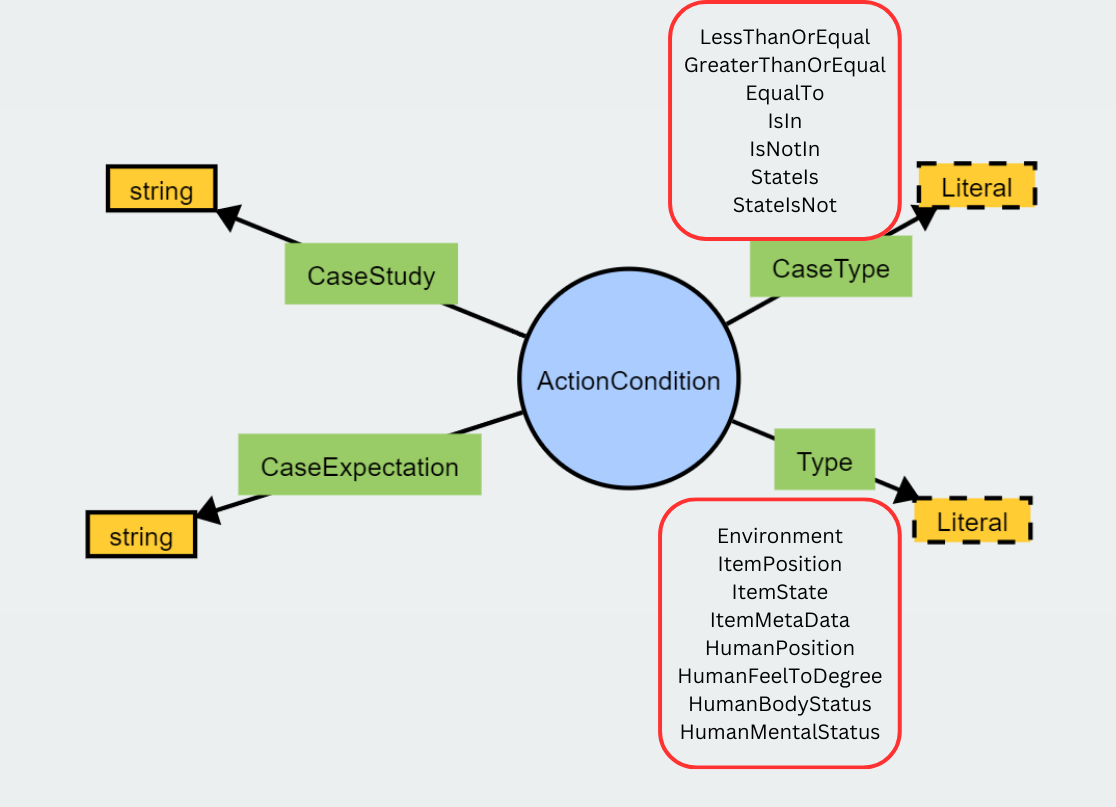
\includegraphics[width=1\textwidth]{figs/f406.png}}
\caption{هستی‌شناسی شرایط فعالیت‌های خانه هوشمند}
\label{fig:f406}
\end{figure}

در هستی‌شناسی نتایج انجام فعالیت که در شکل \ref{fig:f407} قابل مشاهده است، نوع موجودیت برای نتیجه اعمال شده، نام موجودیت، نوع نتیجه اعمال شده با توجه به موجودیت و نتیجه اعمال شده مانند افزایش یا کاهش، تغییر موقعیت مکانی و تغییر حالت به یک مقدار مشخص ذکر شده است. در هر نتیجه انجام فعالیت، آخرین مقادیر دریافتی از حسگرها تغییر می‌کند (به عنوان مثال اگر نتیجه انجام یک فعالیت این باشد که دمای خانه هوشمند پنج درجه افزایش پیدا کند، آخرین مقدار اندازه‌گیری شده توسط حسگر دما، تغییر خواهد کرد).

\begin{figure}[htp]
\centerline{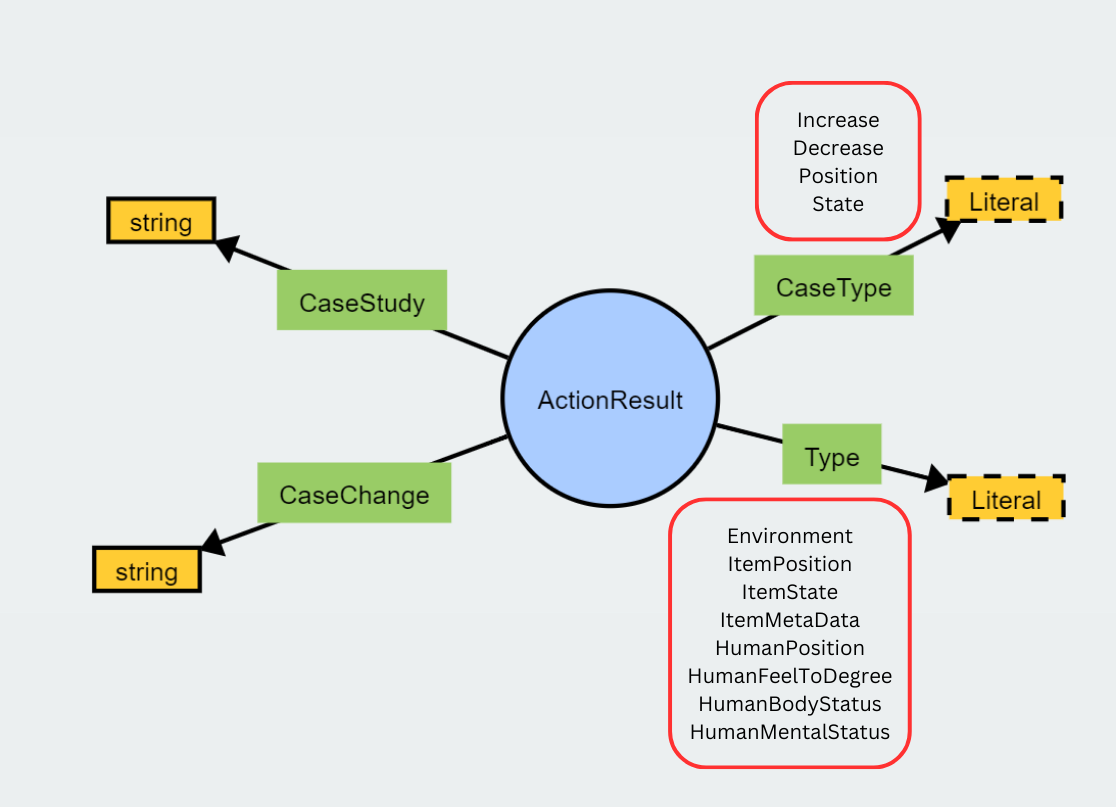
\includegraphics[width=1\textwidth]{figs/f407.png}}
\caption{هستی‌شناسی نتایج فعالیت‌های خانه هوشمند}
\label{fig:f407}
\end{figure}

در هستی‌شناسی فعالیت‌های احتمالی بعدی که در شکل \ref{fig:f408} قابل مشاهده است، تاخیر انجام فعالیت، احتمال انجام و خود فعالیت مشخص شده است.

\begin{figure}[htp]
\centerline{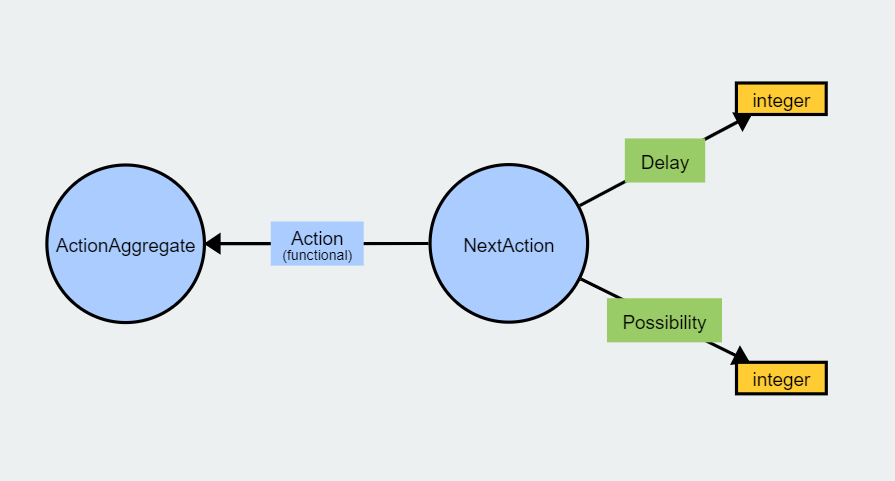
\includegraphics[width=1\textwidth]{figs/f408.png}}
\caption{هستی‌شناسی فعالیت‌های احتمالی بعدی خانه هوشمند}
\label{fig:f408}
\end{figure}

‌\end{itemize}

\subsection{‌مدل‌سازی فعالیت کاربر با قوانین انجمنی}\label{chapter:c442}

در این بخش به مدل‌سازی توالی فعالیت کاربر با استفاده از قوانین انجمنی خواهیم پرداخت و حرکت رو به جلو و رو به عقب سلسله فعالیت‌های کاربر را بررسی خواهیم کرد.

همانطور که در هستی‌شناسی شکل \ref{fig:f408} مشاهده شد؛ هر فعالیت شامل لیستی از فعالیت‌های احتمالی بعدی است که احتمال انجام هر یک با توجه به سوابق کاربر در هستی‌شناسی فعالیت‌ها ثبت شده است. با توجه به قوانین انجمنی مطرح شده در بخش \ref{chapter:c24}، احتمال انجام فعالیت \lr{Y} پس از فعالیت \lr{X} همان اطمینان است که بیان می‌کند در چند درصد مواقع پس از انجام فعالیت \lr{X}، فعالیت \lr{Y} انجام می‌شود. مثالی از نحوه مدل‌سازی احتمال توالی فعالیت‌ها با استفاده از قوانین انجمنی در شکل \ref{fig:f42} قابل مشاهده است (احتمال توالی هر فعالیت پس از فعالیت دیگر به رنگ سبز نشان داده شده است). 

\begin{figure}[htp]
\centerline{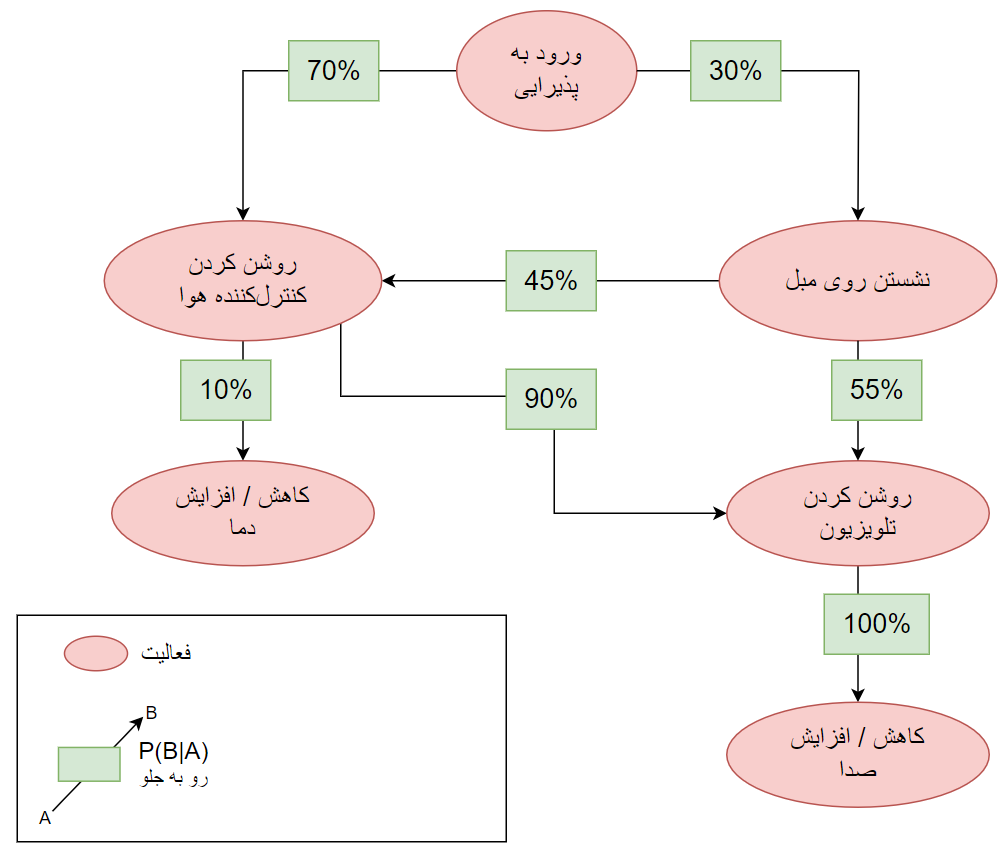
\includegraphics[width=1\textwidth]{figs/f42.png}}
\caption{مثالی از مدل‌سازی احتمال‌ توالی فعالیت‌ها با استفاده از قوانین انجمنی}
\label{fig:f42}
\end{figure}

حال با توجه به مقدار اطمینان و با استفاده از تعریف پشتیبانی برای انجام فعالیت \lr{Y} پس از فعالیت \lr{X}، احتمال انجام فعالیت \lr{X} قبل از فعالیت \lr{Y} با فرض انجام \lr{Y} را تعریف می‌کنیم. این تعریف برای حرکت عقبگرد بین فعالیت‌ها می‌باشد تا بتوانیم انتخاب فعالیت قبل از یک فعالیت مشخص از بین فعالیت‌های ممکن را با دخیل کردن احتمال انجام هر یک انجام دهیم. این احتمال با استفاده از پشتیبانی انجام فعالیت \lr{Y} پس از فعالیت \lr{X} محاسبه می‌شود.

برای انجام محاسبات مربوط به احتمال انتخاب هر فعالیت در حرکت عقبگرد، در ابتدا برای هر فعالیت احتمال رخداد آن به صورت کلی را طبق فرمول زیر محاسبه می‌کنیم:

\begin{equation}
P(X) = \sum_{\text{Parents}} P(\text{Parent}) \cdot P(\text{Parent} \to X)
\end{equation}

در این فرمول، فعالیت‌هایی که به عنوان فعالیت بعدی در هستی‌شناسی هیچ فعالیت دیگری تعریف نشده‌اند، احتمال یک را دارند. برای دیگر فعالیت‌ها مانند فعالیت \lr{X}، تمامی فعالیت‌هایی که پس از آن‌ها فعالیت \lr{X} احتمال انجام دارد را پیدا می‌کنیم (لیست آن فعالیت‌ها را \lr{Parents} می‌نامیم). سپس احتمال رخداد هر فعالیت \lr{Parent} که طبق همین فرمول حساب شده را در احتمال رخداد فعالیت \lr{X} به شرط رخداد فعالیت \lr{Parent} ضرب کرده و در آخر مقدار به دست آمده به ازای هر فعالیت \lr{Parent} را با هم جمع می‌کنیم. در ابتدای هر اجرای ابزار پیشنهادی این پژوهش، احتمال رخداد هر فعالیت به صورت کلی را محاسبه و ذخیره می‌کنیم. احتمال رخداد کلی هر فعالیت در مثال شکل \ref{fig:f42}، در شکل \ref{fig:f42b} قابل مشاهده است (احتمال کلی رخداد هر فعالیت به رنگ بنفش نشان داده شده است).

\begin{figure}[htp]
\centerline{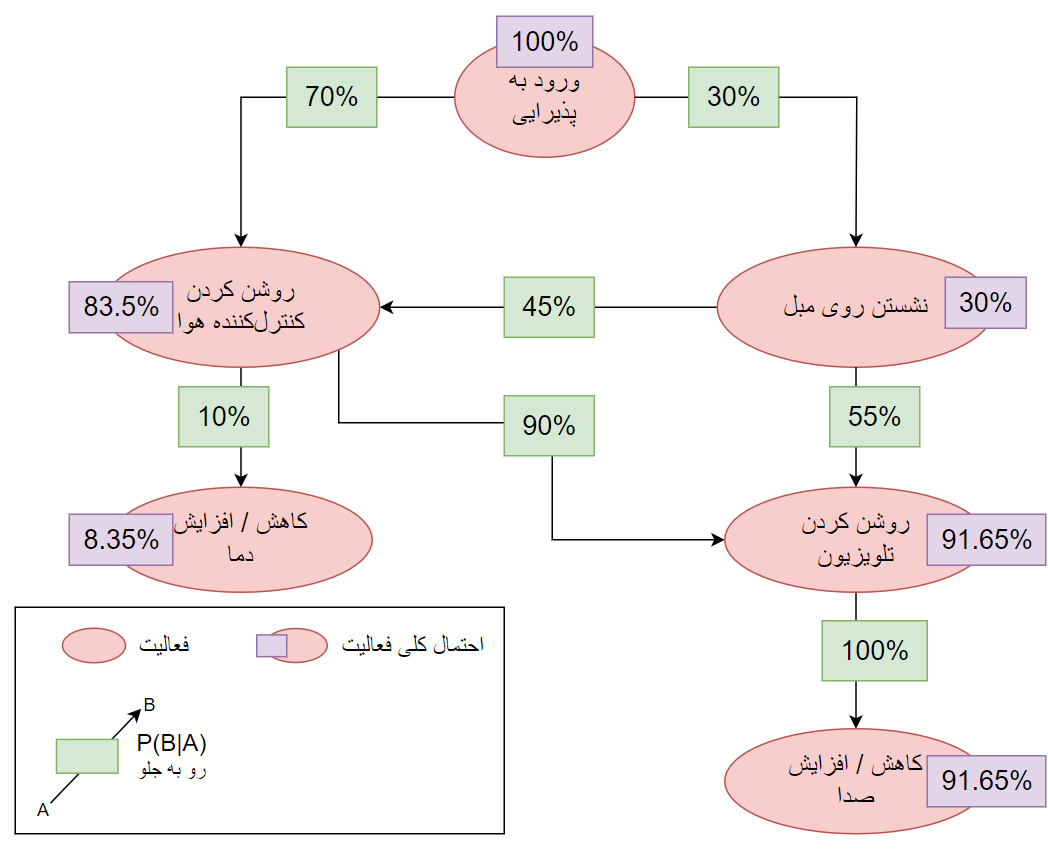
\includegraphics[width=1\textwidth]{figs/f42b.png}}
\caption{احتمال کلی فعالیت‌ها در مثال شکل \ref{fig:f42}}
\label{fig:f42b}
\end{figure}

حال برای احتمال عقبگرد، از فرمول احتمالات شرطی استفاده می‌کنیم:

\begin{equation}
P(Y|X) = \frac{P(X|Y) \cdot P(Y)}{P(X)}
\end{equation}

در این فرمول با استفاده از احتمال رخداد هر فعالیت مانند فعالیت \lr{X} پس از هر فعالیت مانند \lr{Y} و همچنین احتمال رخداد کلی فعالیت‌های \lr{X} و \lr{Y} که محاسبه شده است، احتمال رخداد فعالیت \lr{Y} به صورت حرکت عقبگرد از فعالیت \lr{X} قابل محاسبه است. احتمال انتخاب فعالیت‌ها در حرکت عقبگرد در مثال شکل \ref{fig:f42}، در شکل  \ref{fig:f44} قابل مشاهده است (احتمال انتخاب هر فعالیت برای حرکت عقبگرد از فعالیتی دیگر به رنگ زرد نشان داده شده است).

\begin{figure}[htp]
\centerline{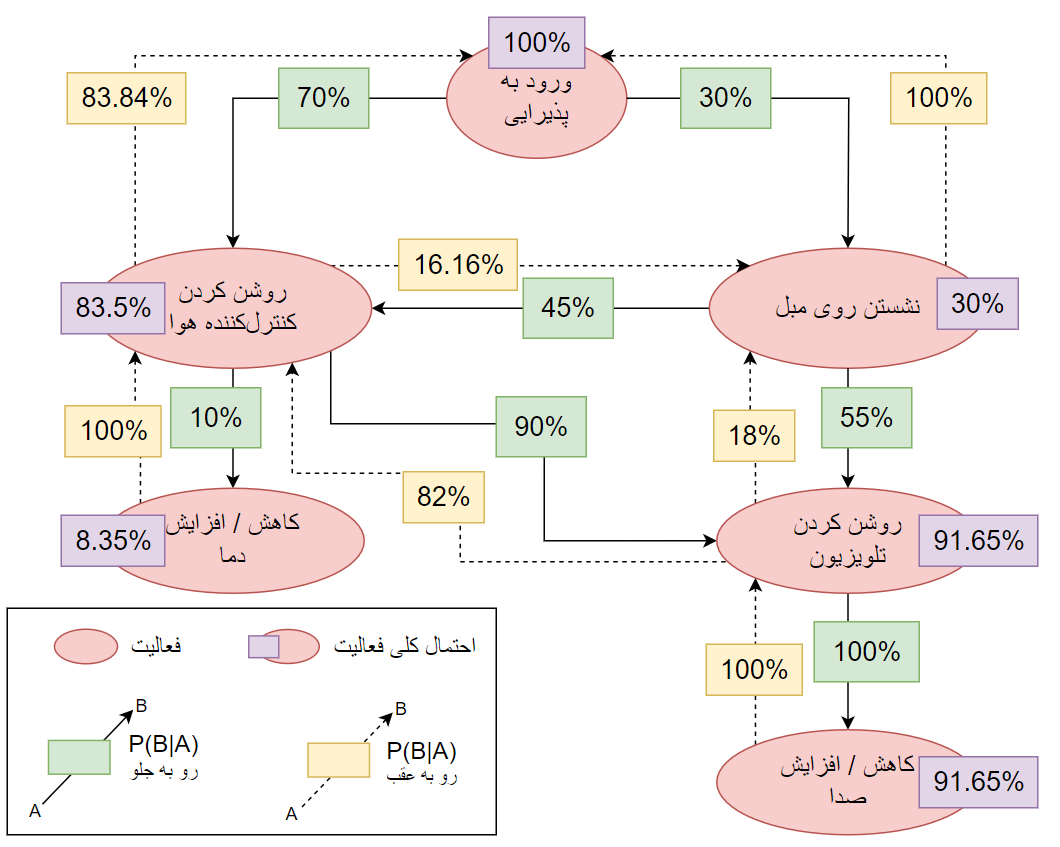
\includegraphics[width=1\textwidth]{figs/f44.png}}
\caption[احتمال انتخاب فعالیت‌ها در حرکت عقبگرد]{احتمال انتخاب فعالیت‌ها در حرکت عقبگرد در مثال شکل \ref{fig:f42}}
\label{fig:f44}
\end{figure}

\subsection{‌الگوریتم تولید سلسله فعالیت جعلی}\label{chapter:c443}

ابزار مبتنی بر راهکار پیشنهادی برای تولید سلسله فعالیت جعلی از الگوریتم نمایش داده شده در شکل \ref{fig:f43} استفاده می‌کند. به طور کلی این فرایند به چند فاز مختلف تقسیم می‌شود که در ادامه به بررسی هر یک خواهیم پرداخت.

\begin{figure}[htp]
\centerline{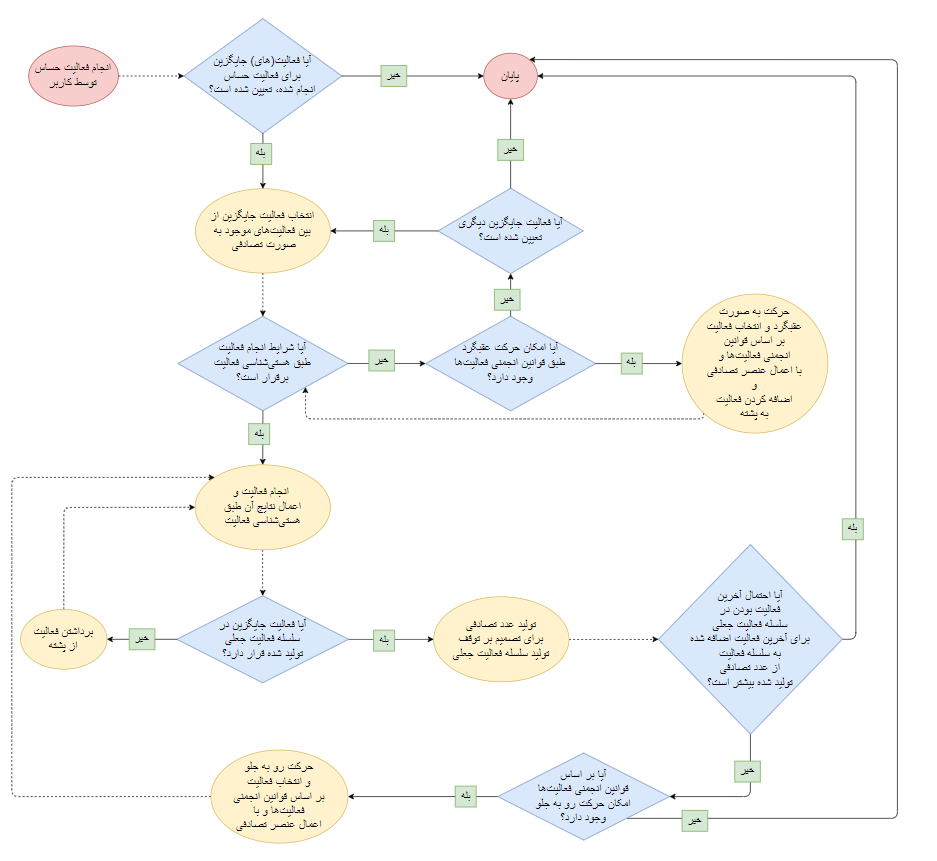
\includegraphics[width=1\textwidth]{figs/f43.png}}
\caption{الگوریتم تولید سلسله فعالیت جعلی}
\label{fig:f43}
\end{figure}

\begin{itemize}
\item \textbf{انجام فعالیت حساس توسط کاربر}: در اولین گام، فعالیتی حساس توسط کاربر انجام می‌شود و ابزار مبتنی بر راهکار پیشنهادی، از بین فعالیت‌های جایگزین برای این فعالیت حساس که توسط کاربر تعیین شده است، یکی را به صورت تصادفی انتخاب کرده و اقدام به تولید سلسله فعالیت جعلی می‌کند که این فعالیت جایگزین در آن حضور داشته باشد.

\item \textbf{حرکت عقبگرد}: حال ابزار مبتنی بر راهکار پیشنهادی، با شروع از فعالیت جایگزین، حرکتی عقبگرد بر اساس قوانین انجمنی را شروع می‌کند تا جایی که به فعالیتی برسد که شرایط انجام آن طبق هستی‌شناسی فعالیت برقرار باشد. در این حرکت عقبگرد تمامی فعالیت‌ها در یک پشته ذخیره می‌شوند تا در صورت ارضا شدن شرایط یک فعالیت، آن‌ها را از پشته برداریم و به سلسله فعالیت جعلی اضافه کنیم. به طور مثال برای «روشن کردن تلویزیون»، ابتدا باید یک فرد در پذیرایی حضور داشته باشد و برای حضور در پذیرایی باید از راهرو به آنجا وارد شد. به همین صورت حرکت عقبگرد انجام می‌دهیم تا به طور واقعی حضور فرد و ارضا شدن دیگر شرایط برای یک فعالیت را داشته باشیم؛ حال فعالیت‌های داخل پشته را برداشته و به سلسله فعالیت جعلی اضافه می‌کنیم. توجه شود که انتخاب فعالیت در حرکت عقبگرد بر اساس قوانین انجمنی و با اعمال عنصر تصادفی است که احتمال انتخاب هر فعالیت با استفاده از محاسبات مطرح شده در بخش \ref{chapter:c442} انجام می‌شود. در صورتی که تمامی مسیرهای طی شده در فعالیت عقبگرد نتیجه‌ای در بر نداشته باشد و هیچ فعالیتی را نتوان به عنوان نقطه شروع انتخاب کرد، به برنامه‌ی مورد استفاده توسط کاربر اعلانی ارسال می‌شود و تولید سلسله فعالیت جعلی با شروع از فعالیت «ورود به خانه» انجام می‌گردد.

\item \textbf{حرکت رو به جلو}: حال که فعالیت جایگزین مورد نظر در سلسله فعالیت جعلی اضافه شده است؛ ابزار مبتنی بر راهکار پیشنهادی برای فریب سکو و یکسان نبودن سلسله فعالیت جعلی برای یک فعالیت جایگزین، حرکتی رو به جلو بر اساس قوانین انجمنی انجام می‌دهد. در ابتدا با استفاده از احتمال توقف آخرین فعالیت که در هستی‌شناسی آمده است تصمیم به ادامه تولید فعالیت جعلی یا توقف می‌گیرد؛ اگر تصمیم بر ادامه تولید فعالیت جعلی گرفته شد، با استفاده از قوانین انجمنی و با اعمال عنصر تصادفی یکی از فعالیت‌های ممکن برای کاربر با استفاده از محاسبات بخش \ref{chapter:c442} را انتخاب کرده و آن را به سلسله فعالیت جعلی اضافه می‌کند. در صورتی که هیچ یک از فعالیت‌های تعیین شده توسط کاربر را نتوان به عنوان فعالیت جعلی تولید کرد، اعلانی به کاربر ارسال می‌گردد تا کاربر فعالیت جایگزین دیگری را تعیین کند و ابزار مبتنی بر راهکار پیشنهادی، الگوریتم تولید سلسله فعالیت جعلی را برای آن فعالیت جایگزین اجرا می‌کند. چنانچه کاربر فعالیت جایگزین جدیدی تعیین نکند، تولید سلسله فعالیت جعلی در آن زمان انجام نمی‌گردد.

\item \textbf{نقطه توقف نهایی}: پس از حرکت رو به جلو جهت فریب سکو، حالت خانه هوشمند را به سمت حالت کنونی واقعی می‌بریم تا از حالات اشیاء و افراد حاضر در خانه پس از مدتی، سکو توانایی تشخیص رخداد سلسله فعالیت جعلی را نداشته باشد. برای این کار آخرین فعالیتی که تاثیر مهمی در حالات افراد حاضر در خانه و اشیاء گذاشته را از داده‌های حسگرها دریافت می‌کنیم، سپس اقدام به تولید مجدد سلسله فعالیت جعلی تا انجام آن فعالیت به عنوان فعالیت نهایی می‌کنیم. پس از تولید هر فعالیت جعلی، آخرین فعالیت با تاثیر مهم را بررسی مجدد می‌کنیم تا به صورت پویا و بدون تولید کامل سلسله فعالیت جعلی، حالت توقف را به حالت واقعی خانه هوشمند نزدیک کنیم. با استفاده از این روش همواره به حالت واقعی خانه هوشمند می‌رسیم که در بدترین حالت که تغییر سریع و مداوم حالت خانه هوشمند است، در هنگام پایان روز و زمان خوابیدن کاربران به حالت واقعی خانه هوشمند می‌رسیم.
‌\end{itemize}

در تولید سلسله فعالیت جعلی، جهت نزدیک بودن به واقعیت، مدت زمان میانگین انجام هر فعالیت را نیز در هستی‌شناسی لحاظ کرده‌ایم. علاوه بر آن، از آنجایی که تمامی موجودیت‌ها در خانه، هوشمند نیستند و ابزار مبتنی بر راهکار پیشنهادی از جزئیات کامل خبر ندارد؛ یک تاخیر بین فعالیت‌ها لحاظ می‌شود که زمان بین اتمام یک فعالیت و شروع فعالیت بعدی است. به طور مثال پس از «ورود به خانه»، «روشن کردن کولر» به طور میانگین پس از دو ثانیه انجام می‌شود که این زمان، حرکت کاربر از درب خانه به سمت کولر و روشن کردن آن است. 

با استفاده از مدت زمان انجام هر فعالیت و فاصله زمانی آن تا فعالیت بعدی، هر فعالیتی که به سلسله فعالیت جعلی اضافه شود؛ یک زمان انجام فعالیت معینی دارد که آن زمان، زمان انجام فعالیت قبلی علاوه بر مدت زمان انجام آن و تاخیر بین فعالیت قبلی و فعالیت کنونی است. به طور مثال اگر «ورود به خانه» به مدت یک ثانیه طول می‌کشد و همچنین میانگین تاخیر بین باز کردن درب خانه و روشن کردن کولر هشت ثانیه باشد؛ زمان انجام فعالیت «روشن کردن کولر» 1 + 8 = 9 ثانیه پس از «ورود به خانه» خواهد بود.

\subsection{‌عوامل تصادفی‌ساز}

از آنجا که سکو قادر به ذخیره و مقایسه‌ی سلسله فعالیت‌ها و همچنین کشف شباهت بین آن‌هاست؛ در تولید سلسله فعالیت جعلی از عوامل تصادفی‌ساز استفاده می‌کنیم تا تنوع در تولید خروجی لحاظ شود. در این بخش به بررسی این عوامل خواهیم پرداخت.

\begin{itemize}
\item \textbf{انتخاب فعالیت جایگزین}: زمانی که فعالیتی حساس انجام می‌شود، فعالیت جایگزین از بین فعالیت‌های جایگزینی که ترجیح کاربر است به طور تصادفی انتخاب می‌شود.
\item \textbf{انتخاب فعالیت در حرکت عقبگرد}: همانطور که اشاره شد، زمانی که به صورت عقبگرد حرکت می‌کنیم، احتمال انتخاب هر فعالیت به صورت تصادفی بوده اما احتمال محاسبه شده در قوانین انجمنی برای حرکت عقبگرد، به عنوان وزن در این انتخاب لحاظ می‌شود. برای این کار برای هر فعالیت سهمی برابر احتمال محاسبه شده در نظر می‌گیریم، سپس عددی تصادفی تولید کرده و با توجه به این که مقدار آن در سهم کدام فعالیت است، فعالیت مورد نیاز را انتخاب می‌کنیم. با این کار علاوه بر لحاظ کردن وزن به دست آمده با استفاده از قوانین انجمنی، از عنصر تصادفی نیز بهره بردیم.

به عنوان مثال، سه فعالیت با احتمال محاسبه شده‌ی 10، 30 و 60 درصد داریم، سهم فعالیت اول بازه 0 تا 10، سهم فعالیت دوم بازه 10 تا 40 و سهم فعالیت سوم بازه 40 تا 100 است. حال عدد تصادفی بین 0 تا 100 تولید می‌کنیم و فعالیت منتخب، فعالیتی خواهد بود که عدد تصادفی تولید شده متعلق به بازه‌ی آن است.
\item \textbf{انتخاب فعالیت در حرکت رو به جلو}: با استفاده از قوانین انجمنی و هستی‌شناسی فعالیت‌ها، برای حرکت رو به جلو فعالیت بعدی در سلسله فعالیت جعلی را به صورت تصادفی انتخاب کرده اما مانند انتخاب فعالیت در حرکت عقبگرد، احتمال انجام فعالیت‌ها در تعیین فعالیت بعدی به صورت تصادفی لحاظ می‌شوند.
\item \textbf{تصمیم توقف}: پس از آن که فعالیت جایگزین در سلسله فعالیت جعلی اضافه شد؛ امکان حرکت رو به جلو یا توقف داریم. این تصمیم با مقدار احتمال توقف که هر فعالیت در هستی‌شناسی خود آن را دارد انجام می‌پذیرد و به صورت وزن‌دار لحاظ می‌شود اما در نهایت این تصمیم به صورت تصادفی بوده و در هر بار اجرا امکان توقف یا حرکت رو به جلو داریم.
\item \textbf{مدت زمان انجام فعالیت و تاخیر بین فعالیت‌ها}: همانطور که اشاره شد، زمان انجام هر فعالیت در سلسله فعالیت جعلی با استفاده از زمان انجام فعالیت قبلی، مدت زمان انجام آن و تاخیر بین این دو فعالیت محاسبه خواهد شد. حال برای آن که فاصله‌ی انجام بین دو فعالیت مشخص همیشه یکسان نباشد، مدت زمان انجام فعالیت‌ها و تاخیر بین انجام فعالیت‌های مختلف در سلسله فعالیت جعلی، با مقداری تصادفی بین حداقل زمان مورد نیاز تا پنج برابر حداقل زمان مورد نیاز جمع زده می‌شوند تا هر بار فاصله‌ی بین انجام فعالیت‌ها نیز متفاوت باشد.
‌\end{itemize}

\section{جمع‌بندی}

در این فصل به طور کامل راهکار پیشنهادی را بررسی کرده و توصیف اجمالی راه حل را ارائه کردیم. برای طراحی هر چه بهتر این نرم‌افزار مدل تهدید را بررسی کرده و بر اساس آن معماری کلان و مدل‌سازی را با جزئیات توصیف کردیم.
